\section{Programmierung}
\subsection{Programmablaufplan}
\vspace{1cm}
\begin{center}
	\tikzstyle{startstop} = [rectangle, rounded corners, minimum width=3cm, minimum height=1cm,text centered, draw=black, fill=red!30]
	\tikzstyle{io} = [trapezium, trapezium left angle=70, trapezium right angle=110, minimum width=3cm, minimum height=1cm, text centered, draw=black, fill=blue!30]
	\tikzstyle{process} = [rectangle, minimum width=3cm, minimum height=1cm, text centered, text width=3cm, draw=black, fill=orange!30]
	\tikzstyle{decision} = [diamond, minimum width=1cm, minimum height=1cm, text centered, text width=3cm, draw=black, fill=green!30]
	\tikzstyle{arrow} = [thick,->,>=stealth]
	\begin{tikzpicture}[node distance=2cm]
		\node (start) [startstop] {Start};
		\node (pro1) [process,below of=start] {Vordefinierter Anfangsweg};
		\node (in1) [io,below of=pro1] {Eingabedaten verarbeiten};
		\node (dec1) [decision,below of=in1,yshift=-1cm] {Roboter aktiv?};
		\node (dec2) [decision,below of=dec1,xshift=3.5cm,yshift=-2cm] {Priorität festlegen};
		\node (pro2) [process,below of=dec1,xshift=-4cm,yshift=-2cm] {Herausfahrvektor berechnen};
		\node (pro3) [process,below of=dec2,xshift=-4cm,yshift=-1.5cm] {Verfolgungsvektor berechnen};
		\node (pro4) [process,below of=dec2,xshift=4cm,yshift=-1.5cm] {Fliehvektor berechnen};
		\node (pro5) [process,below of=pro3,xshift=4cm,yshift=-1cm] {Vektor anpassen};
		\node (in2) [io,below of=pro5] {Befehle senden};
		
		\draw [arrow] (start) -- (pro1);
		\draw [arrow] (pro1) -- (in1);
		\draw [arrow] (in1) -- (dec1);
		\draw [arrow] (dec1) -| node[anchor=south] {ja} (dec2);
		\draw [arrow] (dec1) -| node[anchor=south] {nein} (pro2);
		\draw [arrow] (dec2) -| node[anchor=south] {fangen} (pro3);
		\draw [arrow] (dec2) -| node[anchor=south] {fliehen} (pro4);
		\draw [arrow] (pro2) |- (pro5);
		\draw [arrow] (pro3) -| (pro5);
		\draw [arrow] (pro4) -| (pro5);
		\draw [arrow] (pro5) -- (in2);
		\draw [arrow] (in2) -| (10.5, -8) |- (0,-3);
	\end{tikzpicture}
\end{center}
\newpage
\subsection{Hauptformular}
\begin{center}
	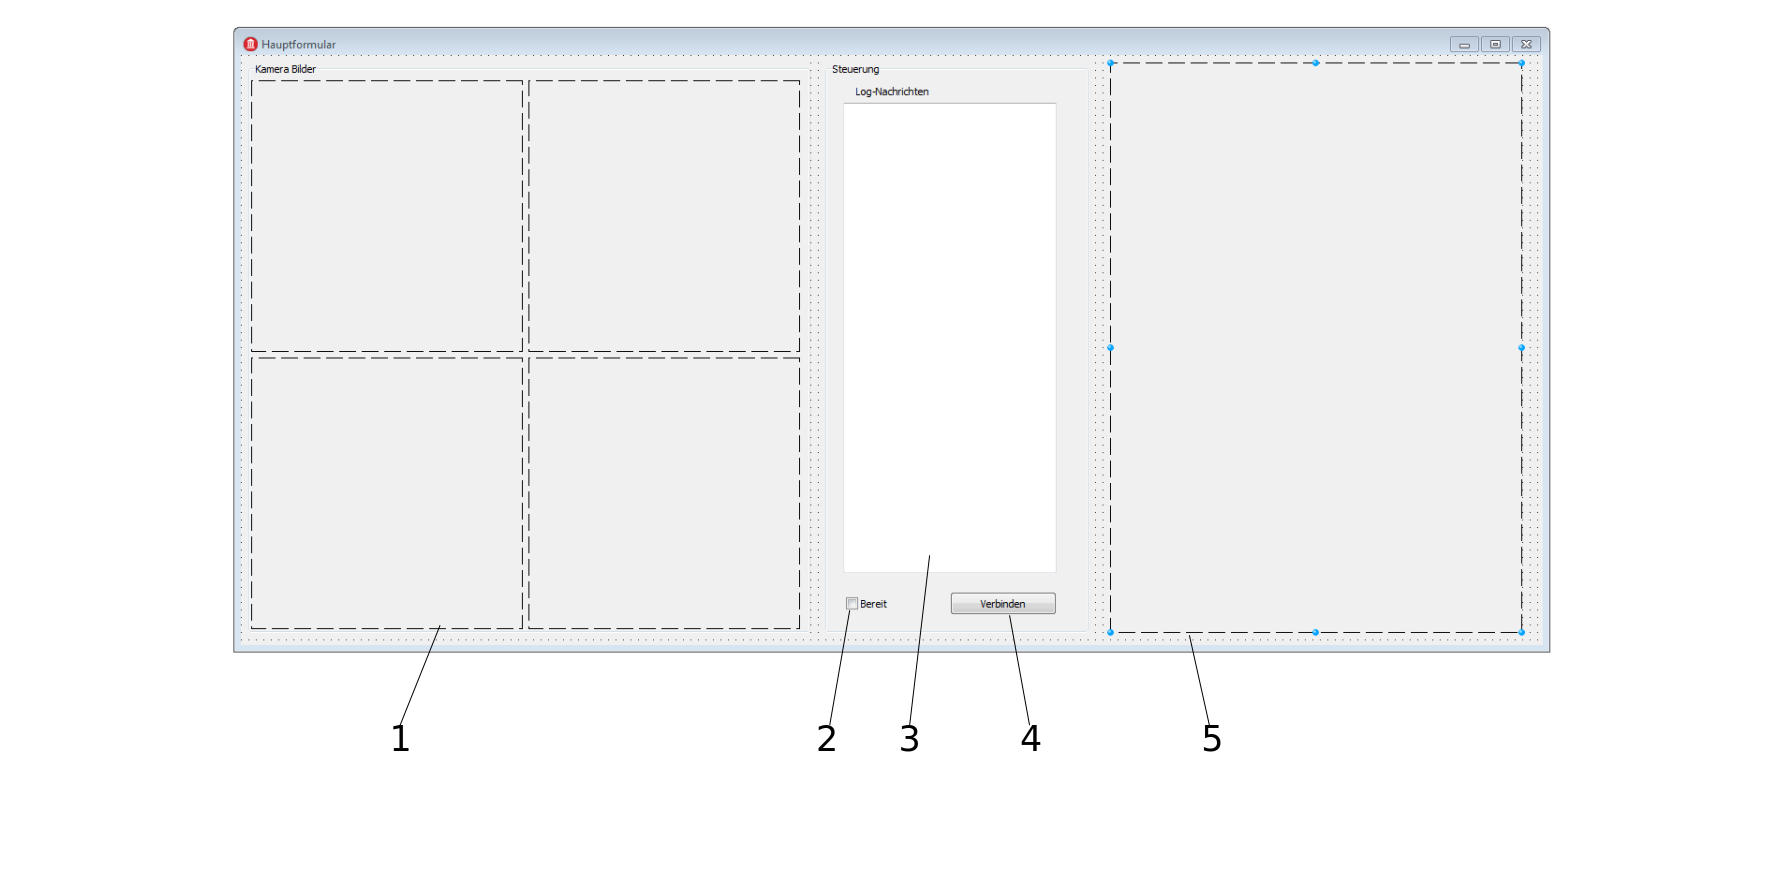
\includegraphics[scale=0.4]{Bilder/GUI.pdf}
\end{center}
\begin{enumerate}
	\item Anzeige der Bilder, von den USB-Kameras der Roboter 
	\item Kontrollkästchen, das der Roboter bereit ist
	\item Anzeige von Fehler-, Hinweis- und Warnmeldungen
	\item Schaltknopf zum Verbinden der Roboter mit dem Server
	\item Grafische Anzeige der Bewegung, von den einzelnen Robotern\\
\end{enumerate}
\textbf{Prozeduren:}
\begin{description}
	\item[Ereignisprotokoll] Hinweis-, Fehler- und Warnmeldungen werden in einer Ereignisprotokolldatei abgespeichert, sowie in einem Listenfeld \textbf{"'3"'} angezeigt.
	\item[KamerabilderAnzeigen] Es werden die Bilder der USB-Kameras der Roboter in den Feldern \textbf{"'1"'} angezeigt.
	\item[Visualisierung] In dem Feld \textbf{"'5"'} werden die Bewegungen unserer Roboter grafisch dargestellt.
	\item[FormCreate] In der FormCreate wird das Fenster für das Programm erstellt. Außerdem werden in der FormCreate die IP-Adressen aus einer IP-Config.txt Datei eingelesen und in einem Array abgelegt, dass für die spätere Verbindung zum Server benötigt wird.
\end{description}

\subsection{Klassen}
Für die Berechnungen und Logik haben wir eigene Klassen geschrieben.\\
\newline
Diese unterteilen sich in:
\begin{itemize}
	\item mVektor
	\item mTKI
	\item mKonstanten
	\item mRoboterDaten
\end{itemize}

\subsubsection{mVektor}
Die Klasse mVektor besteht aus dem Record TVektor.
\\
Dieser hat folgende Funktionen, überladende Operatoren und Variablen:
%\newline
%\textbf{Funktionen:}\\
%\newline
%\begin{tabulary}{\textwidth}{|l|l|l|l|}
%	\hline
%	\textbf{Arbeitspaket} & \textbf{AP-Nr.:} & \textbf{Arbeitspaketverantwortlicher} & \bf{Beteiligte Personen}\\
%	\multirow{2}{1cm}{Winkel (überladen)} & 1.1.1 & Sven Stegemann & Eugen Zwetzich\\
%	& & &\\
%	\hline
%	\multicolumn{4}{|l|}{\textbf{Ergebniss:}}\\
%	\multicolumn{4}{|l|}{- Winkel in Bogenmaß}\\
%	\multicolumn{4}{|l|}{}\\
%	\multicolumn{4}{|l|}{\textbf{Aufgabenstellung:}}\\
%	\multicolumn{4}{|p{\textwidth}|}{Es wird der Winkel, zwischen dem Vektor und der X-Achse berechnet und im halboffenen Intervall $[0;2\pi)$ als Bogenmaß zurück gegeben.}\\
%	\hline
%\end{tabulary}
%\\
%\newline
%\\
%\begin{tabulary}{1\linewidth}{|l|l|l|l|}
%	\hline
%	\textbf{Arbeitspaket} & \textbf{AP-Nr.:} & \textbf{Arbeitspaketverantwortlicher} & \bf{Beteiligte Personen}\\
%	\multirow{2}{1cm}{Winkel (überladen)} & 1.1.2 & Sven Stegemann & Eugen Zwetzich\\
%	& & &\\
%	\hline
%	\multicolumn{4}{|l|}{\textbf{Ergebniss:}}\\
%	\multicolumn{4}{|l|}{- Winkel in Bogenmaß}\\
%	\multicolumn{4}{|l|}{}\\
%	\multicolumn{4}{|l|}{\textbf{Aufgabenstellung:}}\\
%	\multicolumn{4}{|p{\textwidth}|}{Es wird der Winkel zwischen zwei Vektoren berechnet und als Bogenmaß zurückgegeben.}\\
%	\hline
%\end{tabulary}
%\\
%\newline
%\\
%\begin{tabulary}{1\linewidth}{|l|l|l|l|}
%	\hline
%	\textbf{Arbeitspaket} & \textbf{AP-Nr.:} & \textbf{Arbeitspaketverantwortlicher} & \bf{Beteiligte Personen}\\
%	Betrag & 1.1.3 & Sven Stegemann & Eugen Zwetzich\\
%	\hline
%	\multicolumn{4}{|l|}{\textbf{Ergebniss:}}\\
%	\multicolumn{4}{|l|}{- Länge des Vektors}\\
%	\multicolumn{4}{|l|}{}\\
%	\multicolumn{4}{|l|}{\textbf{Aufgabenstellung:}}\\
%	\multicolumn{4}{|p{\textwidth}|}{Es wird die euklidische Norm(2-Norm) des Vektors gebildet.}\\
%	\hline
%\end{tabulary}
%\\
%\newline
%\\
%\begin{tabulary}{1\linewidth}{|l|l|l|l|}
%	\hline
%	\textbf{Arbeitspaket} & \textbf{AP-Nr.:} & \textbf{Arbeitspaketverantwortlicher} & \bf{Beteiligte Personen}\\
%	Drehen & 1.1.4 & Sven Stegemann & Michael Mertens\\
%	\hline
%	\multicolumn{4}{|l|}{\textbf{Ergebniss:}}\\
%	\multicolumn{4}{|l|}{- Vektor um Winkel gedreht}\\
%	\multicolumn{4}{|l|}{}\\
%	\multicolumn{4}{|l|}{\textbf{Aufgabenstellung:}}\\
%	\multicolumn{4}{|p{\textwidth}|}{Mit der Drehmatrix wird ein neuer Vektor berechnet, der um einen als Parameter übergebenen Winkel nach links(positiv) bzw. nach rechts(negativ) gedreht ist.}\\
%	\hline
%\end{tabulary}
%\\
%\newline
%\\
%\textbf{Operatoren:}\\
%\newline
%\begin{tabulary}{1\linewidth}{|l|l|l|l|}
%	\hline
%	\textbf{Arbeitspaket} & \textbf{AP-Nr.:} & \textbf{Arbeitspaketverantwortlicher} & \bf{Beteiligte Personen}\\
%	Add & 1.2.1 & Sven Stegemann & Eugen Zwetzich\\
%	\hline
%	\multicolumn{4}{|l|}{\textbf{Ergebniss:}}\\
%	\multicolumn{4}{|l|}{- Summe zweier Vektoren}\\
%	\multicolumn{4}{|l|}{}\\
%	\multicolumn{4}{|l|}{\textbf{Aufgabenstellung:}}\\
%	\multicolumn{4}{|p{\textwidth}|}{Es werden komponentenweise zwei Vektoren addiert und ein neuer Vektor wird zurück gegeben.}\\
%	\hline
%\end{tabulary}
%\\
%\newline
%\\
%\begin{tabulary}{1\linewidth}{|l|l|l|l|}
%	\hline
%	\textbf{Arbeitspaket} & \textbf{AP-Nr.:} & \textbf{Arbeitspaketverantwortlicher} & \bf{Beteiligte Personen}\\
%	Substract & 1.2.2 & Sven Stegemann & Eugen Zwetzich\\
%	\hline
%	\multicolumn{4}{|l|}{\textbf{Ergebniss:}}\\
%	\multicolumn{4}{|l|}{- Differenz zweier Vektoren}\\
%	\multicolumn{4}{|l|}{}\\
%	\multicolumn{4}{|l|}{\textbf{Aufgabenstellung:}}\\
%	\multicolumn{4}{|p{\textwidth}|}{Es werden komponentenweise zwei Vektoren subtrahiert und ein neuer Vektor wird zurück gegeben.}\\
%	\hline
%\end{tabulary}
%\\
%\newline
%\\
%\begin{tabulary}{1\linewidth}{|l|l|l|l|}
%	\hline
%	\textbf{Arbeitspaket} & \textbf{AP-Nr.:} & \textbf{Arbeitspaketverantwortlicher} & \bf{Beteiligte Personen}\\
%	\multirow{2}{1cm}{Multiply (überladen)} & 1.2.3 & Sven Stegemann & Eugen Zwetzich\\
%	& & &\\
%	\hline
%	\multicolumn{4}{|l|}{\textbf{Ergebniss:}}\\
%	\multicolumn{4}{|l|}{- Vektor}\\
%	\multicolumn{4}{|l|}{}\\
%	\multicolumn{4}{|l|}{\textbf{Aufgabenstellung:}}\\
%	\multicolumn{4}{|p{\textwidth}|}{Es werden die einzelnen Komponenten des Vektors mit einem Skalar multipliziert und ein neuer Vektor zurück gegeben.}\\
%	\hline
%\end{tabulary}
%\\
%\newline
%\\
%\begin{tabulary}{1\linewidth}{|l|l|l|l|}
%	\hline
%	\textbf{Arbeitspaket} & \textbf{AP-Nr.:} & \textbf{Arbeitspaketverantwortlicher} & \bf{Beteiligte Personen}\\
%	\multirow{2}{1cm}{Multiply (überladen)} & 1.2.4 & Sven Stegemann & Eugen Zwetzich\\
%	& & &\\
%	\hline
%	\multicolumn{4}{|l|}{\textbf{Ergebniss:}}\\
%	\multicolumn{4}{|l|}{- Skalar}\\
%	\multicolumn{4}{|l|}{}\\
%	\multicolumn{4}{|l|}{\textbf{Aufgabenstellung:}}\\
%	\multicolumn{4}{|p{\textwidth}|}{Es wird ein Skalar mit den einzelnen Komponenten eines Vektors multiplieziert und ein Skalar zurück gegeben.}\\
%	\hline
%\end{tabulary}
%\\
%\newline
%\\
%\begin{tabulary}{1\linewidth}{|l|l|l|l|}
%	\hline
%	\textbf{Arbeitspaket} & \textbf{AP-Nr.:} & \textbf{Arbeitspaketverantwortlicher} & \bf{Beteiligte Personen}\\
%	Equal & 1.2.5 & Sven Stegemann & Eugen Zwetzich\\
%	\hline
%	\multicolumn{4}{|l|}{\textbf{Ergebniss:}}\\
%	\multicolumn{4}{|l|}{- True oder False}\\
%	\multicolumn{4}{|l|}{}\\
%	\multicolumn{4}{|l|}{\textbf{Aufgabenstellung:}}\\
%	\multicolumn{4}{|p{\textwidth}|}{Es wird überprüft ob die Komponenten zweier Vektoren gleich sind.}\\
%	\hline
%\end{tabulary}
%\\
%\newline
%\\
%\textbf{Variablen:}\\
%\newline
%\begin{tabulary}{1\linewidth}{|l|l|l|l|}
%	\hline
%	\textbf{Arbeitspaket} & \textbf{AP-Nr.:} & \textbf{Arbeitspaketverantwortlicher} & \bf{Beteiligte Personen}\\
%	x,y & 1.3.1 & Sven Stegemann & Eugen Zwetzich\\
%	\hline
%	\multicolumn{4}{|l|}{\textbf{Ergebniss:}}\\
%	\multicolumn{4}{|l|}{- }\\
%	\multicolumn{4}{|l|}{}\\
%	\multicolumn{4}{|l|}{\textbf{Aufgabenstellung:}}\\
%	\multicolumn{4}{|p{\textwidth}|}{x, y sind die Komponenten eines Vektors.}\\
%	\hline
%\end{tabulary}

\begin{itemize}
	\item Funktionen
	\begin{description}
		\item[Winkel(überladen)] Berechnet den Winkel zwischen dem Vektor und der X-Achse. Als Rückgabewert erhält man einen Wert im Bogenmaß im Intervall von [0;$2\pi$).
		\item[Winkel(überladen)] Berechnet den Winkel zwischen zwei Vektoren. Als Rückgabewert erhält man einen Wert im Bogenmaß im Intervall von [0;$2\pi$). 
		\item[Betrag] Es wird die Länge des Vektors(euklidische Norm: 2-Norm) berechnet.
		\item[Drehen] Mit der Drehmatrix wird ein neuer Vektor berechnet, der um einen als Parameter übergebenen Winkel nach links(positiv) bzw. nach rechts(negativ) gedreht ist. 
	\end{description}
	\item Operatoren
	\begin{description}
		\item[Add] Es werden die Komponenten der jeweiligen Vektoren addiert und anschließend ein neuer Vektor zurück gegeben.
		\item[Substract] Es werden die Komponenten der jeweiligen Vektoren subtrahiert und anschließend ein neuer Vektor zurück gegeben.
		\item[Multiply(überladen)] Es werden die einzelnen Komponenten des Vektors mit einem Skalar multipliziert und ein neuer Vektor zurück gegeben.
		\item[Multiply(überladen)] Es wird ein Skalar mit den Komponenten eines Vektors multipliziert und ein Skalar zurück gegeben.
		\item[Equal] Es werden die einzelnen Komponenten zweier Vektoren auf Gleichheit überprüft.
	\end{description}
	\item Variablen
	\begin{description}
		\item[x,y] sind die Komponenten eines Vektors.
	\end{description}
\end{itemize}

\subsubsection{mTKI}
Die Klasse mTKI hat einen Datentypen TAktion mit den Werten Fliehen und Fangen und eine abgeleitete Klasse TKI von TObject.

Die abgeleitete Klasse TKI besteht aus foglenden Funktionen, Prozeduren und Variablen:\\
\newline
\textbf{Funktionen:}\\
\newline
\begin{tabulary}{1\textwidth}{|l|l|l|l|}
	\hline
	\textbf{Arbeitspaket} & \textbf{AP-Nr.:} & \textbf{Arbeitspaketverantwortlicher} & \bf{Beteiligte Personen}\\
	\multirow{2}{1cm}{Prioritat Festlegen} & 2.1.1 & Sven Stegemann & Eugen Zwetzich\\
	& & &\\
	\hline
	\multicolumn{4}{|l|}{\textbf{Ergebniss:}}\\
	\multicolumn{4}{|l|}{-FLIEHEN}\\
	\multicolumn{4}{|l|}{-FANGEN}\\
	\multicolumn{4}{|l|}{}\\
	\multicolumn{4}{|l|}{\textbf{Aufgabenstellung:}}\\
	\multicolumn{4}{|p{\textwidth}|}{Anhand der Positionsdaten der gegnerischen Roboter wird überprüft, welcher sich am nächsten an unserem Roboter befindet. Anschließend wird über die Winkel Funktion von der Klasse mVektor ermittelt, ob sich dieser Roboter vor oder hinter unserem befindet. Danach wird die Priorität auf FLIEHEN bzw. auf FANGEN gesetzt.}\\
	\hline
\end{tabulary}
\\
\newline
\\
\begin{tabulary}{1\textwidth}{|l|l|l|l|}
	\hline
	\textbf{Arbeitspaket} & \textbf{AP-Nr.:} & \textbf{Arbeitspaketverantwortlicher} & \bf{Beteiligte Personen}\\
	\multirow{2}{1cm}{Fangvektor Berechnen} & 2.1.2 & Sven Stegemann & Jonah Vennemann\\
	& & &\\
	\hline
	\multicolumn{4}{|l|}{\textbf{Ergebniss:}}\\
	\multicolumn{4}{|l|}{-Vektor}\\
	\multicolumn{4}{|l|}{}\\
	\multicolumn{4}{|l|}{\textbf{Aufgabenstellung:}}\\
	\multicolumn{4}{|p{\textwidth}|}{Es wird der Vektor zum nächsten gegnerischen Roboter, der Gefangen werden soll, berechnet. Als Rückgabewert erhält man einen neuen Vektor.}\\
	\hline
\end{tabulary}
\\
\newline
\\
\begin{tabulary}{1\textwidth}{|l|l|l|l|}
	\hline
	\textbf{Arbeitspaket} & \textbf{AP-Nr.:} & \textbf{Arbeitspaketverantwortlicher} & \bf{Beteiligte Personen}\\
	\multirow{2}{1cm}{Fliehvektor Berechnen} & 2.1.3 & Sven Stegemann & Michael Mertens\\
	& & &\\
	\hline
	\multicolumn{4}{|l|}{\textbf{Ergebniss:}}\\
	\multicolumn{4}{|l|}{-Vektor}\\
	\multicolumn{4}{|l|}{}\\
	\multicolumn{4}{|l|}{\textbf{Aufgabenstellung:}}\\
	\multicolumn{4}{|p{\textwidth}|}{Es wird ein Vektor, mit Bezug auf den gegnerischen Roboter von dem Geflohen werden soll, berechnet. Als Rückgabewert erhält man einen neuen Vektor.}\\
	\hline
\end{tabulary}
\\
\newline
\\
\begin{tabulary}{1\textwidth}{|l|l|l|l|}
	\hline
	\textbf{Arbeitspaket} & \textbf{AP-Nr.:} & \textbf{Arbeitspaketverantwortlicher} & \bf{Beteiligte Personen}\\
	\multirow{3}{2cm}{Rand Ausweichvektor Berechnen} & 2.1.4 & Sven Stegemann & Michael Mertens\\
	& & &\\
	& & &\\
	\hline
	\multicolumn{4}{|l|}{\textbf{Ergebniss:}}\\
	\multicolumn{4}{|l|}{-Vektor}\\
	\multicolumn{4}{|l|}{}\\
	\multicolumn{4}{|l|}{\textbf{Aufgabenstellung:}}\\
	\multicolumn{4}{|p{\textwidth}|}{Es wird überprüft ob sich der Roboter im Spielfeld befindet ist dieser außerhalb, so fährt er sofort in's Spielfeld rein. Danach wird überprüft ob sich der Roboter in der Nähe des Spielfeldrandes befindet. Ist dieser zu Nah am Spielfeldrand, wird der Roboter nach links bzw. nach rechts gedreht.}\\
	\hline
\end{tabulary}
\\
\newline
\\
\begin{tabulary}{1\textwidth}{|l|l|l|l|}
	\hline
	\textbf{Arbeitspaket} & \textbf{AP-Nr.:} & \textbf{Arbeitspaketverantwortlicher} & \bf{Beteiligte Personen}\\
	\multirow{4}{2cm}{Roboter Ausweichvektor Berechnen} & 2.1.5 & Sven Stegemann & Michael Mertens\\
	& & &\\
	& & &\\
	& & &\\
	\hline
	\multicolumn{4}{|l|}{\textbf{Ergebniss:}}\\
	\multicolumn{4}{|l|}{-Vektor}\\
	\multicolumn{4}{|l|}{}\\
	\multicolumn{4}{|l|}{\textbf{Aufgabenstellung:}}\\
	\multicolumn{4}{|p{\textwidth}|}{Es wird geprüft welche Roboter aus unserem Team untereinander kollidieren würden. Wurde ein Roboter ermittelt, so wird dieser um die Konstante AUSWEICHWINKEL gedreht. Als Rückgabewert erhält man einen neuen Vektor.}\\
	\hline
\end{tabulary}
\\
\newline
\\
\begin{tabulary}{1\textwidth}{|l|l|l|l|}
	\hline
	\textbf{Arbeitspaket} & \textbf{AP-Nr.:} & \textbf{Arbeitspaketverantwortlicher} & \bf{Beteiligte Personen}\\
	\multirow{2}{1cm}{Rausfahrvektor Berechnen} & 2.1.6 & Sven Stegemann & Michael Mertens\\
	& & &\\
	\hline
	\multicolumn{4}{|l|}{\textbf{Ergebniss:}}\\
	\multicolumn{4}{|l|}{-Vektor}\\
	\multicolumn{4}{|l|}{}\\
	\multicolumn{4}{|l|}{\textbf{Aufgabenstellung:}}\\
	\multicolumn{4}{|p{\textwidth}|}{Sobald ein Roboter als "`Gefangen"' gemeldet ist, wird anhand seiner Position und der Spielfeldgröße ein Vektor zum Herausfahren berechnet. Als Rückgabewert erhält man einen neuen Vektor.}\\
	\hline
\end{tabulary}
\\
\newline
\\
\begin{tabulary}{1\textwidth}{|l|l|l|l|}
	\hline
	\textbf{Arbeitspaket} & \textbf{AP-Nr.:} & \textbf{Arbeitspaketverantwortlicher} & \bf{Beteiligte Personen}\\
	\multirow{2}{1cm}{Serverdaten Empfangen} & 2.1.7 & Sven Stegemann & Michael Mertens\\
	& & &\\
	\hline
	\multicolumn{4}{|l|}{\textbf{Ergebniss:}}\\
	\multicolumn{4}{|l|}{-}\\
	\multicolumn{4}{|l|}{}\\
	\multicolumn{4}{|l|}{\textbf{Aufgabenstellung:}}\\
	\multicolumn{4}{|p{\textwidth}|}{So bald sich der Client mit dem Server verbunden hat, werden die Variablen des Roboters mit Daten vom Server gefüllt.}\\
	\hline
\end{tabulary}
\\
\newline
\\
\begin{tabulary}{1\textwidth}{|l|l|l|l|}
	\hline
	\textbf{Arbeitspaket} & \textbf{AP-Nr.:} & \textbf{Arbeitspaketverantwortlicher} & \bf{Beteiligte Personen}\\
	Anmelden & 2.1.8 & Sven Stegemann & Michael Mertens\\
	\hline
	\multicolumn{4}{|l|}{\textbf{Ergebniss:}}\\
	\multicolumn{4}{|l|}{-}\\
	\multicolumn{4}{|l|}{}\\
	\multicolumn{4}{|l|}{\textbf{Aufgabenstellung:}}\\
	\multicolumn{4}{|p{\textwidth}|}{Ist eine Funktion um sich mit dem Server zu verbinden.}\\
	\hline
\end{tabulary}
\\
\\
\newline
\textbf{Prozeduren:}\\
\newline
\begin{tabulary}{1\textwidth}{|l|l|l|l|}
	\hline
	\textbf{Arbeitspaket} & \textbf{AP-Nr.:} & \textbf{Arbeitspaketverantwortlicher} & \bf{Beteiligte Personen}\\
	\multirow{2}{1cm}{Steuerbefehl Senden} & 2.2.1 & Sven Stegemann & Eugen Zwetzich\\
	& & &\\
	\hline
	\multicolumn{4}{|l|}{\textbf{Ergebniss:}}\\
	\multicolumn{4}{|l|}{-}\\
	\multicolumn{4}{|l|}{}\\
	\multicolumn{4}{|l|}{\textbf{Aufgabenstellung:}}\\
	\multicolumn{4}{|p{\textwidth}|}{Als erstes wird überprüft ob der aktuelle Vektor oder der Zielvektor ein Nullvektor ist. Danach wird ermittelt ob der aktuelle Vektor sich links bzw. rechts vom Roboter befindet. Zum Schluss wird dem Roboter eine Standardgeschwindigkeit übergeben.}\\
	\hline
\end{tabulary}
\\
\newline
\\
\begin{tabulary}{1\textwidth}{|l|l|l|l|}
	\hline
	\textbf{Arbeitspaket} & \textbf{AP-Nr.:} & \textbf{Arbeitspaketverantwortlicher} & \bf{Beteiligte Personen}\\
	\multirow{2}{1cm}{Geschwindigkeit Berechnen} & 2.2.2 & Sven Stegemann & Michael Mertens\\
	& & &\\
	\hline
	\multicolumn{4}{|l|}{\textbf{Ergebniss:}}\\
	\multicolumn{4}{|l|}{-}\\
	\multicolumn{4}{|l|}{}\\
	\multicolumn{4}{|l|}{\textbf{Aufgabenstellung:}}\\
	\multicolumn{4}{|p{\textwidth}|}{Es wird von dem Vektor Geschwindigkeit, die Geschwindigkeit in $\frac{m}{s}$ berechnet.}\\
	\hline
\end{tabulary}
\\
\newline
\\
\begin{tabulary}{1\textwidth}{|l|l|l|l|}
	\hline
	\textbf{Arbeitspaket} & \textbf{AP-Nr.:} & \textbf{Arbeitspaketverantwortlicher} & \bf{Beteiligte Personen}\\
	\multirow{2}{1cm}{Initialisierung} & 2.2.3 & Sven Stegemann & Michael Mertens\\
	& & &\\
	\hline
	\multicolumn{4}{|l|}{\textbf{Ergebniss:}}\\
	\multicolumn{4}{|l|}{-}\\
	\multicolumn{4}{|l|}{}\\
	\multicolumn{4}{|l|}{\textbf{Aufgabenstellung:}}\\
	\multicolumn{4}{|p{\textwidth}|}{Anhand der IP-Adressen, wird jeweils ein Roboter von der Klasse TTXTMobilRoboter erstellt. Ist keine Verbindung möglich, so wird ein Fehler in die Log-Datei geschrieben.}\\
	\hline
\end{tabulary}
\\
\newline
\\
\begin{tabulary}{1\textwidth}{|l|l|l|l|}
	\hline
	\textbf{Arbeitspaket} & \textbf{AP-Nr.:} & \textbf{Arbeitspaketverantwortlicher} & \bf{Beteiligte Personen}\\
	Steuern & 2.2.4 & Sven Stegemann & Michael Mertens\\
	\hline
	\multicolumn{4}{|l|}{\textbf{Ergebniss:}}\\
	\multicolumn{4}{|l|}{-}\\
	\multicolumn{4}{|l|}{}\\
	\multicolumn{4}{|l|}{\textbf{Aufgabenstellung:}}\\
	\multicolumn{4}{|p{\textwidth}|}{Ist eine Funktion um sich mit dem Server zu verbinden.}\\
	\hline
\end{tabulary}

\subsubsection{mKonstanten}
Da wir an verschiedenen Stellen die gleichen Werte benötigten, erstellten wir eine eigene Klasse für Konstanten.
%\newline
%\textbf{Konstanten:}\\
%\newline
%\begin{tabulary}{\textwidth}{|l|l|l|l|}
%	\hline
%	\textbf{Arbeitspaket} & \textbf{AP-Nr.:} & \textbf{Arbeitspaketverantwortlicher} & \bf{Beteiligte Personen}\\
%	Mindestabstand & 3.1.1 & Eugen Zwetzich & Sven Stegemann\\
%	\hline
%	\multicolumn{4}{|l|}{\textbf{Ergebniss:}}\\
%	\multicolumn{4}{|l|}{-}\\
%	\multicolumn{4}{|l|}{}\\
%	\multicolumn{4}{|l|}{\textbf{Aufgabenstellung:}}\\
%	\multicolumn{4}{|p{\textwidth}|}{Ist die Position eines einzelnen Roboters als Vektor.}\\
%	\hline
%\end{tabulary}
%\\
%\newline
%\\
%\begin{tabulary}{\textwidth}{|l|l|l|l|}
%	\hline
%	\textbf{Arbeitspaket} & \textbf{AP-Nr.:} & \textbf{Arbeitspaketverantwortlicher} & \bf{Beteiligte Personen}\\
%	Nullvektor & 3.1.2 & Eugen Zwetzich & Sven Stegemann\\
%	\hline
%	\multicolumn{4}{|l|}{\textbf{Ergebniss:}}\\
%	\multicolumn{4}{|l|}{-}\\
%	\multicolumn{4}{|l|}{}\\
%	\multicolumn{4}{|l|}{\textbf{Aufgabenstellung:}}\\
%	\multicolumn{4}{|p{\textwidth}|}{Ist die Position eines einzelnen Roboters als Vektor.}\\
%	\hline
%\end{tabulary}
%\\
%\newline
%\\
%\begin{tabulary}{\textwidth}{|l|l|l|l|}
%	\hline
%	\textbf{Arbeitspaket} & \textbf{AP-Nr.:} & \textbf{Arbeitspaketverantwortlicher} & \bf{Beteiligte Personen}\\
%	Rand & 3.1.2 & Eugen Zwetzich & Sven Stegemann\\
%	\hline
%	\multicolumn{4}{|l|}{\textbf{Ergebniss:}}\\
%	\multicolumn{4}{|l|}{-}\\
%	\multicolumn{4}{|l|}{}\\
%	\multicolumn{4}{|l|}{\textbf{Aufgabenstellung:}}\\
%	\multicolumn{4}{|p{\textwidth}|}{Ist die Position eines einzelnen Roboters als Vektor.}\\
%	\hline
%\end{tabulary}
%\\
%\newline
%\\
%\begin{tabulary}{\textwidth}{|l|l|l|l|}
%	\hline
%	\textbf{Arbeitspaket} & \textbf{AP-Nr.:} & \textbf{Arbeitspaketverantwortlicher} & \bf{Beteiligte Personen}\\
%	Ausweichwinkel & 3.1.2 & Eugen Zwetzich & Sven Stegemann\\
%	\hline
%	\multicolumn{4}{|l|}{\textbf{Ergebniss:}}\\
%	\multicolumn{4}{|l|}{-}\\
%	\multicolumn{4}{|l|}{}\\
%	\multicolumn{4}{|l|}{\textbf{Aufgabenstellung:}}\\
%	\multicolumn{4}{|p{\textwidth}|}{Ist die Position eines einzelnen Roboters als Vektor.}\\
%	\hline
%\end{tabulary}
%\\
%\newline
%\\
%\begin{tabulary}{\textwidth}{|l|l|l|l|}
%	\hline
%	\textbf{Arbeitspaket} & \textbf{AP-Nr.:} & \textbf{Arbeitspaketverantwortlicher} & \bf{Beteiligte Personen}\\
%	\multirow{2}{1cm}{Länge Fliehvektor} & 3.1.2 & Eugen Zwetzich & Sven Stegemann\\
%	& & &\\
%	\hline
%	\multicolumn{4}{|l|}{\textbf{Ergebniss:}}\\
%	\multicolumn{4}{|l|}{-}\\
%	\multicolumn{4}{|l|}{}\\
%	\multicolumn{4}{|l|}{\textbf{Aufgabenstellung:}}\\
%	\multicolumn{4}{|p{\textwidth}|}{Ist die Position eines einzelnen Roboters als Vektor.}\\
%	\hline
%\end{tabulary}
\begin{itemize}
	\item Variablen
	\begin{itemize}
		\item Mindestabstand
		\item Nullvektor
		\item Rand
		\item Ausweichwinkel
		\item LängeFliehvektor
	\end{itemize}
\end{itemize}

\subsubsection{mRoboterDaten}
Um den Zugriff auf die Daten eines Roboters zu vereinfachen, haben wir diese in einer eigenen Klasse mRoboterDaten untergebracht.
\\
Diese besteht aus einem Record TRoboterDaten mit folgenden Variablen:
\\\\
\textbf{Variablen:}
\begin{itemize}
	\item Position
	\item Geschwindigkeit
	\item Positionsverlauf
	\item Aktiv
\end{itemize}


